\documentclass[pdf]{beamer}
\usepackage[utf8]{vietnam}
\usepackage{amsmath}
\usepackage{amssymb}
\usepackage[utf8]{inputenc}
\usepackage{algorithm,algorithmic}
\usepackage{subfig}
\usepackage{color}
\usepackage{colortbl}
\mode<presentation>{\usetheme{Madrid}}
%\usecolortheme{whale}

%% preamble
\title{Biterm Topic Model}
%\subtitle{Mô hình Biterm}
\author{Nguyễn Bá Cương}
\institute[]
{
	School of Information and Communication Technology
	Hanoi University of Science and Technology\\
}
\date[VLC 2017] % (optional)
{Data Science Lab , 2017}
\begin{document}

%% title frame
\begin{frame}
\titlepage
\end{frame}

\begin{frame}{Nội dung}
\tableofcontents
\end{frame}

\AtBeginSection[]
{
\begin{frame}{Nội dung}
\tableofcontents[currentsection]
\end{frame}
}

%%%%%%%%%%%%%%%%%%%%%%%%%%%%%%%%%%%%%%%%%%%
\section{Short texts và mô hình chủ đề}
\subsection{Short texts}
\begin{frame}{Gới thiệu về short texts}
	Những văn bản ngắn rất là phổ biến trên các trang web 
	\begin{figure}
		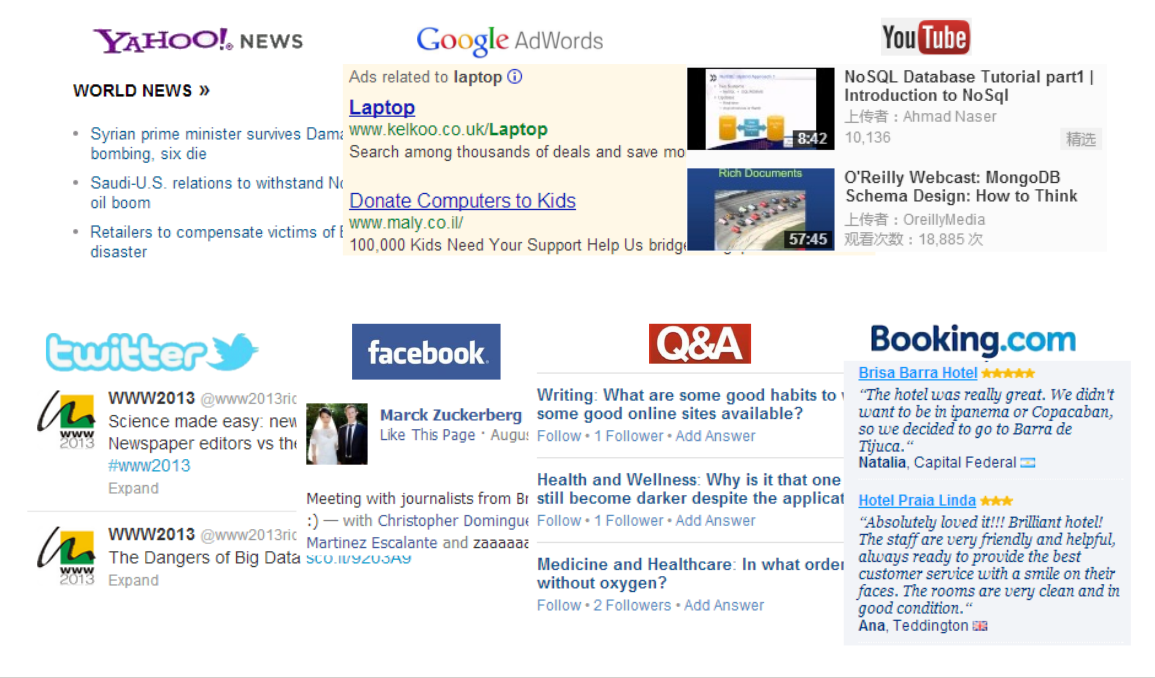
\includegraphics[width=1\textwidth]{01.png}
	\end{figure}
\end{frame}

\begin{frame}{Ứng dụng của short texts}
Hiểu được chủ đề của các văn bản ngắn rất là quan trong trong nhiều lĩnh vực
	\begin{itemize}
		\item Mô tả đặc điểm nội dung (content characterizing)
		\item Gợi ý nội dung (content recommendation)
		\item Sở thích người dùng (user interest profiling)
		\item Phát hiện các chủ đề nổi lên (emerging topic detecting)
		\item Phân tích ngữ nghĩa (semantic analysic)
		\item ...
	\end{itemize}
\end{frame}

\begin{frame}{Những vần đề của short texts}
	Những khó khăn và thách thức
	\begin{itemize}
		\item Không đủ ngữ cảnh để xác định ý nghĩa của câu
		\item Các đặc điểm short texts
		\begin{itemize}
			\item Độ dài văn bản rất ngắn
			\item Số lượng dữ liệu của văn bản ngắn là rất lớn và tăng nhanh
			\item Các chủ để nó phản ánh đến các xu hướng xã hội
		\end{itemize}
		\item Việc giới hạn độ dài của văn bản trong short texts làm cho chúng rất khó để phân tích với các mô hình xác suất truyền thống
	\end{itemize}

\end{frame}

\subsection{Các mô hình chủ đề}
\begin{frame}{Mô hình chủ đề}
\begin{figure}
	\subfloat[Mô hình chủ đề]{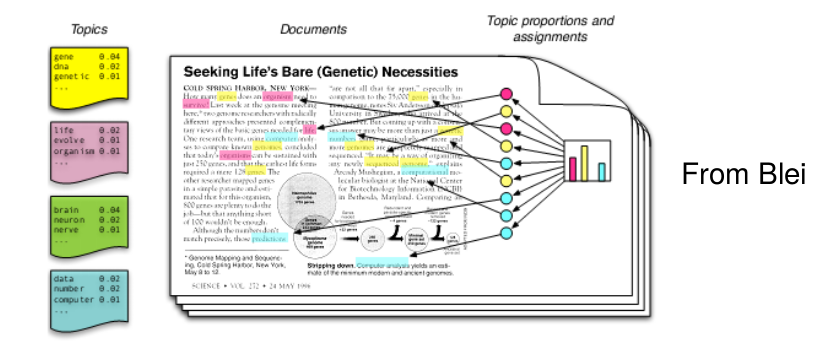
\includegraphics[width=0.7\textwidth]{02.png}}
\end{figure}
Mô hình sinh của các văn bản với chủ đề ẩn
\begin{itemize}
	\item Một chủ đề $\sim$ một phân phối xác suất trong tập từ vững
	\item Một văn bản $\sim$ một tập trộn của các chủ đề ẩn
	\item Một từ $\sim$ một điểm trong một chủ đề
\end{itemize}	
\end{frame}

\begin{frame}{Mô hình LDA}
	Mô hình sinh của mô hình LDA với $K$ chủ đề.
	\begin{columns}[T] % align columns
		\begin{column}{.55\textwidth}
			\begin{itemize}
				\item  Sinh các phân phối từ theo chủ đề \\
					$1.$ Với một chủ đề $i$ trong trong $K$ \\
				\space $a).$ Lấy mẫu $\beta_i \sim Dir(\eta)$
				\item  Sinh các từ của một văn bản \\
				$1.$ Chọn phân phối trộn các chủ đề của văn bản $\theta \sim Dir(\alpha)$ \\
				$2.$ Ứng với một từ $w_n$ trong văn bản \\
					$a).$ Chọn một chủ đề $z_n \sim Mul(\theta)$ \\
					$b).$ Chọn ra một từ $ w_n \sim Mul(\beta_{z_n})$  \\
			\end{itemize}
		\end{column} %
		\hfill%	
		\begin{column}{.43\textwidth}
			\begin{figure}
				\subfloat[Mô hình LDA]{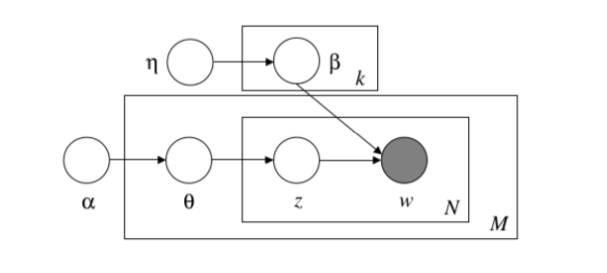
\includegraphics[width=1.15\textwidth]{03.png}}
			\end{figure}				
		\end{column} %
	\end{columns}
\end{frame}
\begin{frame}{LDA cho short texts}
	\begin{itemize}
		\item Vấn đề: 
		\begin{itemize}
			\item Độ dài văn bản ngắn, các từ hầu như chỉ xuất hiện một lần
			\item Không đủ ngữ cảnh để xác định nội dung
		\end{itemize}
	\end{itemize}		
	\begin{itemize}
		\item Một số giải pháp:
		\begin{itemize}
			\item Khái thác kiến thức từ bên ngoài để làm giàu sự biểu diễn cho short texts
			\item Kết hợp một số văn bản ngắn thành một văn bản dài dựa trên một số thông tin. Như tập hợp các bài đăng trên Twitter bời cùng người người dùng...
		\end{itemize}
	\end{itemize}
\end{frame}

\begin{frame}{Mô hình mixture of unigrams}
%	Mô hình sinh của mô hình mixture of unigrams
\begin{columns}[T] % align columns
	\begin{column}{.50\textwidth}
		\begin{itemize}
			\item Giả định rằng tất cả các từ thuộc một văn bản đều thuộc cùng một chủ đề\\
			=> Vấn đề: Mặc dù là short text nhưng mỗi văn bản vẫn có thể có nhiều hơn 1 chủ đề
%			\item trong khi chủ đề $z$ được lấy mẫu từ một tỉ lệ chủ đề toàn cục $\theta$
		\end{itemize}
	\end{column} %
	\hfill%	
	\begin{column}{.50\textwidth}
		\begin{figure}
			\subfloat[Mô hình Mixture of unigrams]{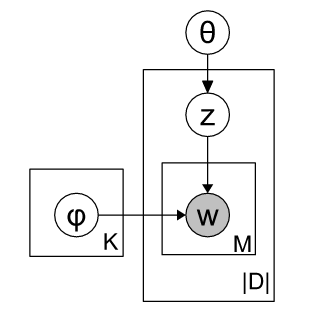
\includegraphics[width=0.85\textwidth]{Mix.png}}
		\end{figure}				
	\end{column} %
\end{columns}
$\hspace{5cm}$
\end{frame}


%%%%%%%%%%%%%%%%%%%%%%%%%%%%%%%%%%%%%%%%%%%
\section{Mô hình Biterm}
\subsection{Giới thiệu về mô hình biterm topic model (BTM)}
\begin{frame}{Ý tưởng}
	\begin{itemize}
		\item Chủ đề cơ bản là một nhóm các từ tương quan với nhau và những từ tương quan với nhau này được phát hiện bởi sự đồng xuất hiện trong một văn bản.  \\
		$\overrightarrow{} $ Tại sao không tồn tại mô hình đồng thời xuất hiện các từ để học từng chủ đề
		\item Mô hình chủ đề cho short texts chịu nhiều ảnh hưởng của dữ liệu thưa \\
		$\overrightarrow{} $  Tại sao không sử dụng toàn bộ nguồn dữ liệu để học ra các chủ đề
	\end{itemize}
\end{frame}

\begin{frame}{Xây dựng biterm và dữ liệu học}
	\begin{itemize}
		\item Biterm là một cặp từ không theo thứ tự cùng xuất hiện trong một văn bản \\
		\centering Ví dụ như một văn bản gồn có 3 từ $w_1, w_2, w_3$ thì biterm là \\
		\centering $(w_1, w_2, w_3) \overrightarrow{} \{(w_1, w_2), (w_2, w_3), (w_1, w_3)\} $
		\item Dữ liệu học bao gồm tất cả các biterm được sinh ra từ bộ dữ liệu ban đầu
	\end{itemize}
\end{frame}

\begin{frame}{Mô hình Biterm Topics Model (BTM)}
	Mô hình sinh của BTM
	\begin{columns}[T] % align columns
		\begin{column}{.55\textwidth}
			\begin{itemize}
				\item Vời từng chủ đề $z$ \\
				$a). $ Lấy mẫu $\phi_z \sim Dir(\beta)$
				\item Chọn phân phối chủ đề $\theta \sim Dir(\alpha)$ cho toàn bộ tập dữ liệu
				\item Với từng biterm $b$ \\
				$a). $ Chọn một phân phối chủ đề \\ 
					$z \sim Mutil(\theta)$ \\
				$b). $ Chọn phân phối các từ trong biterm \\
				\centering $w_1, w_2 \sim Mutil(\phi_z)$
			\end{itemize}
		\end{column} %
		\hfill%	
		\begin{column}{.43\textwidth}
			\begin{figure}
				\subfloat[Mô hình BTM]{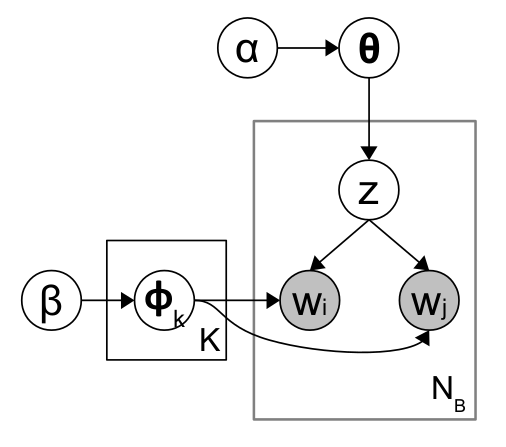
\includegraphics[width=1\textwidth]{BTM.png}}
			\end{figure}				
		\end{column} %
	\end{columns}

\end{frame}

\begin{frame}{Mô hình BTM}
	\begin{figure}
		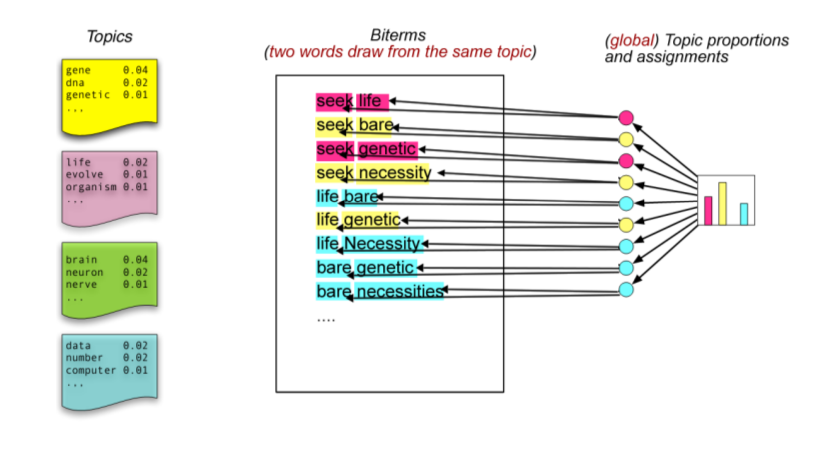
\includegraphics[width=0.65\textwidth]{06.png}
	\end{figure}				
	Mô hình sinh của biterms với chủ đề ẩn
	\begin{itemize}
		\item Chủ đề $\sim$ phân phối qua các từ 
		\item Tập dữ liệu $\sim$ tập trộn các chủ đề
		\item Một biterm $\sim$ hai từ xác định biểu diển cùng trong một chủ đề
	\end{itemize}
\end{frame}
%\subsection{Suy diễn các chủ đề cho từng văn bản}
\begin{frame}{Suy diễn chủ đề cho từng văn bản}
\begin{itemize}
	\item Giả định \\
	Tỉ lệ chủ đề của một văn bản tương đương với kì vọng tỉ lệ chủ đề của các biterm trong văn bản đó.\\
%	Giả sử văn bản $d$ có $N_d$ biterms,$\{b_i^{(d)}\}_{i=1}^{N_d}$
%	\begin{align*}
%		P(z|d) = \sum_{i = 1}^{N_d} P(z,b_i^{(d)}|d) = \sum_{i = 1}^{N_d} P(z|b_i^{(d)})P(b_i^{(d)}|d)
%	\end{align*}

	\begin{align*}
		P(z|d) = \sum_b P(z|b)P(b|d)
	\end{align*}
	\item Trong đó 
	\begin{align*}
		P(z|b) = \dfrac{P(z)P(w_|z)P(w_j|z)}{\sum_zP(z)P(w_i|z)P(w_j|z)}\\
		P(b|d) = \dfrac{n_d(b)}{\sum_bn_d(b)}
	\end{align*}
%	\begin{align*}
%		P(z = k|b_i^{(d)}) = \dfrac{\theta_k \phi_{k, w_{i,1}^{(d)}} \phi_{k, w_{i,2}^{(d)}}}{\sum_{k`}\theta_{k^`} \phi_{k^`, w_{i,1}^{(d)}} \phi_{k^`, w_{i,2}^{(d)}}} \\
%		P(b_i^{(d)}|d) = \dfrac{n(b_i^{(d)})}{\sum_{i=1}^{N_d}n(b_i^{(d)})}
%	\end{align*}
\end{itemize}
\end{frame}
\subsection{Các phương pháp suy diễn}
\begin{frame}{Maximum A Posteriori}
\begin{columns}
	\column{0.5\textwidth}
	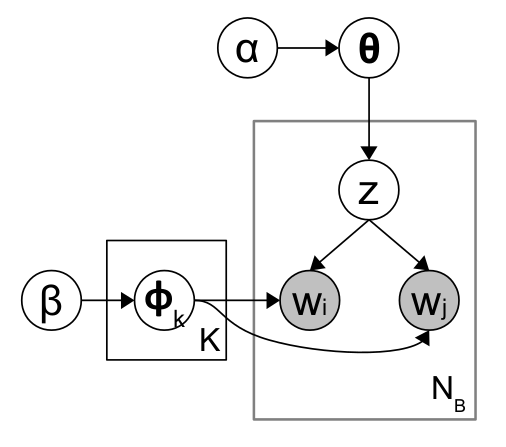
\includegraphics[width=\textwidth]{BTM.png}
	\column{0.5\textwidth}
	\begin{itemize}
		\item $\alpha, \beta$ là hyperparameter. Ta xác định giá trị của nó bằng cross-validation
		\item $Z$ là biến ẩn, chúng ta không quan sát được
		\item Tập các biterm $B$ là dữ liệu duy nhất chúng ta quan sát được
		\item $\Phi, \Theta$ là biến chúng ta cần tìm
	\end{itemize}
\end{columns}
Sử dụng ước lượng MAP:
\begin{align}
\Phi, \Theta =& \text{argmax\ } \log P(\Phi, \Theta | \alpha, \beta, B) \nonumber \\
=& \text{argmax\ } \log P(B | \Phi, \Theta) P(\Phi, \Theta | \alpha, \beta)
\end{align}
\end{frame}

\begin{frame}{Phương pháp Gibbs Sampling}
\begin{itemize}
	\item Ý tưởng: Sinh ra một mẫu phân bố hậu nghiệm bằng cách duyệt qua các giá trị từ tập dữ liêu ban đầu.
	\item Ví dụ:\\
	Cho các biến ngẫu nhiên $X_1, X_2, X_3$\\
	Khởi tạo: $x_1^{(0)}, x_2^{(0)}, x_3^{(0)}$ \\
	Tại bước lặp thứ $i$
	\begin{align*}
	x_1^{(i)} = p(X_1 = x_1| X_2 = x_2^{(i-1)},  X_3 = x_3^{(i-1)})\\
	x_2^{(i)} = p(X_2 = x_2| X_1 = x_1^{(i)},  X_3 = x_3^{(i-1)}) \\
	x_3^{(i)} = p(X_3 = x_3| X_1 = x_1^{(i)},  X_2 = x_2^{(i)}) 
	\end{align*}
	Qúa trình này sẽ dừng đến khi hội tụ
\end{itemize}
\end{frame}

\begin{frame}{Suy diễn tham số}
Lấy mẫu chủ đề cho từng biterm trong mini-batch $t$
\begin{align}
P(z_i = k|z_{-i}^{(t)}, B^{(t)}, \alpha^{(t)}, \{\beta_k^{(t)}\}_{k=1}^K) \propto  \nonumber \\
(n_{-i, k} ^{(t)}, \alpha_k^{(t)})\dfrac{(n_{-i, w_i|k}^{(t)} + \beta_{k, w_i}^{(t)})(n_{-i, w_j|k}^{(t)} + \beta_{k, w_j}^{(t)})}{[\sum_{w=1}^W(n_{-i, w|k}^{(t)} + \beta_{k, w}^{(t)})]^2} 
\end{align}
Cập nhật lại các tham số
\begin{align}
\alpha_k^{(t+1)} = \alpha_k^{(t)} + \lambda n_k^{(t)} \\
\beta_{k, w}^{(t+1)} = \beta_{k, w} ^{(t)} + \lambda n_{w|k}^{(t)} \\
\phi_{k,w}^{(t)} = \dfrac{n_{w|k}^{(t)} + \beta^{(t)}}{n_{.|k}^{(t)} + W\beta^{(t)}} \\
\theta_k^{(t)} = \dfrac{n_k^{(t)} + \alpha^{(t)}}{N_\beta^{(t)} + K\alpha^{(t)}}
\end{align}
\end{frame}

\begin{frame}
\begin{algorithm}[H]
\textbf{Input: }  $K, \alpha , \beta, $ biterm sets $B^{(1)}, ..., B^{(T)}$  \\
\textbf{Output:} $\{\phi^{(t)}, \theta^{(t)} \}_{t=1}^T$
\begin{algorithmic}[1]
\STATE {Set $\alpha^{(1)} = {(\alpha, ..., \alpha)}$ and $\{\beta_k^{(1)} = {(\beta, ..., \beta)}\}_{k = 1}^K$}
\FOR{$t =1$ to $T$ do}
\STATE {Randomly initialize the topic asignments for all the biterms}
\FOR{$iter=1$ to $N_{iter}$ do}
\FOR{\textbf{each} biterm $b_i = {(w_{i, 1}, w_{i,2})} \ni B^{(t)} $}
\STATE {Drawn topic k from Eq.(2)}
\STATE {Update $n_k^{(t)}, n_{w_{i,1}|k}^{(t)}$ and $n_{w_{i,2}|k}^{(t)}$}
\ENDFOR
\STATE {$\alpha^{(t+1)}$ and $\{\beta_k^{(t+1)}\}_{k=1}^{K}$ by Eq.(3)and Eq.(4)}
\ENDFOR
\STATE {Compute $\phi^{(t)}$ by Eq.(5) and $\theta^{(t)}$ by Eq.(6)}
\ENDFOR
\end{algorithmic}
\caption{Thuật toán Gibbs sampling dạng online cho mô hình BTM }
\label{alg:seq}
\end{algorithm}
\end{frame}

\subsection{Phương pháp học mới}
\begin{frame}{Vấn đề và phương pháp học mới}
	\begin{itemize}
		\item Dữ liệu biterm sinh ra quá lớn\\
		=> Việc sử dụng phương pháp Gibbs sampling không hiệu quả và tốn nhiều thời gian
		\item Phương pháp học mới \\
		- Phương pháp học VB \\
		- Phương pháp học ngẫu nhiên trên bộ dữ liệu
	\end{itemize} 
\end{frame}

\begin{frame}{Tư tưởng của Expectation - Maximization}
\begin{itemize}
	\item Ước lượng MAP (1) trong trường hợp này rất khó khăn và không có công thức cụ thể \\
	=>  ta xây dựng một lower-bound cho hàm mục tiêu này và tối ưu hóa trên lower-bound này
	\item Tư tưởng thuật toán. \\
	Giả sử mô hình có tham số $\theta$, biến quan sát được $X$ và tập các biến ẩn $Z$
	=> Sử dụng ước lượng MAP ta có:
	\begin{align}
	\theta_{MAP} & = \text{argmax } \prod_{i}^{N} P(x_{i}|\theta)P(\theta) \nonumber \\
	& = \text{argmax } \sum_{i}^{N} \log P(x_{i}|\theta) + \log P(\theta ) \nonumber  \\
	& = \text{argmax } \sum_{i}^{N} \log \sum_{z_{i}} P(x_{i}z_{i}|\theta) + \log P(\theta ) \label{eq:MAP}
	\end{align}
\end{itemize}


\end{frame}

\begin{frame}{Tư tưởng thuật toán EM}
Với mỗi giá trị $i$, gọi $Q(z_{i})$ là một phân phối trên biến ẩn $z_{i}$, áp dụng bất đẳng thức Jensen ta có:
	\begin{align*}
	& \sum_{i}^{N} \log \sum_{z_{i}} P(x_{i}z_{i}|\theta) + \log P(\theta ) \nonumber \\
	= & \sum_{i}^{N} \log \sum_{z_{i}} Q(z_{i}) \frac{P(x_{i}z_{i}|\theta)}{Q(z_{i})} + \log P(\theta ) \nonumber \\
	\geq & \sum_{i}^{N} \sum_{z_{i}} Q(z_{i}) \log \frac{P(x_{i}z_{i}|\theta)}{Q(z_{i})} + \log P(\theta) \label{eq:jensen}
	= \mathcal{L}(Q,\theta)
	\end{align*}
	
	Dấu bằng khi:
	\begin{align*}
	 Q(z_{i}) \propto P(z_{i}|x_{i},\theta)
	\end{align*}
\end{frame}
\begin{frame}{Tư tưởng thuật toán EM}
Hàm lower-bound:
\begin{align*}
\mathcal{L}(Q, \theta) = & \sum_i^N \sum_{z_{i}} P(z_{i}|x_{i},\theta^{old}) \log P(x_{i}z_{i}|\theta) \\
& - \sum_i^N \sum_{z_{i}} P(z_{i}|x_{i},\theta^{old}) \log P(z_{i}|x_{i},\theta^{old}) + \log P(\theta)
\end{align*}
\begin{itemize}
	\item Bước E 
	\begin{equation*}
	\text{Xác định } \mathcal{Q}(\theta) = \sum_i^N \sum_{z_{i}} P(z_{i}|x_{i},\theta^{old}) \log P(x_{i}z_{i}|\theta) + \log P(\theta)
	\label{eq:Estep}
	\end{equation*}

	\item Bước M
	\begin{equation*}
	\text{Tính } \theta^{new} = \text{argmax}_{\theta} \mathcal{Q}(\theta)
	\label{eq:Mstep}
	\end{equation*}
\end{itemize}
\end{frame}
\begin{frame}{Áp dụng thuật toán cho mô hình BTM}
  Bước E ta tính giá trị
	\begin{align*}
	t_{n,k} &= P(z_{n} = k |b_{n},\theta,{\Phi})\\
	&= P(z_{n} = k |w_{n,1}, w_{n,2},\theta,{\Phi})\\
	&= \frac{P(w_{n,1}, w_{n,2}|z_{n}=k,\theta, {\Phi}) P(z_{n} = k | \theta, {\Phi})}
	{\sum_k P(w_{n,1}, w_{n,2}|z_{n}=k,\theta, {\Phi}) P(z_{n} = k | \theta, {\Phi})}\\
	&= \frac{\phi_{k,w_{n,1}} \phi_{k,w_{n,2}} \theta_k}
	{\sum_k \phi_{k,w_{n,1}} \phi_{k,w_{n,2}} \theta_k}
	\end{align*}
	Bước M ta cập nhật giá trị
	\begin{align*}
	\theta_k &= \frac{\sum_n t_{n,k} + \alpha}{\sum_{k'} \big( \sum_n t_{n,k'} + \alpha \big)} \\
	\phi_{k,w} &= \frac{\sum_{n} t_{n,k} \ c(b_{n},w) + \beta}{W \beta + \sum_{n} 2t_{n,k}}
	\end{align*}
\end{frame}

\begin{frame}
\begin{algorithm}[H]
	Define $ \gamma_i = (i+2)^{-p}$ \\
	\textbf{Input: } topic number $K, \alpha, \beta,$ biterm sets $B^{(1)}, ..., B^{(T)}$  \\
	\textbf{Output: } $\phi, \theta$ 
	\begin{algorithmic}[1]
		\STATE Randomly initialize $\phi, \theta,  S_{\theta_k}^0 = 0, S_{\phi_{k, w}}^0 = 0, i = 0$
		\FOR{$i=1$ to $\infty$}
		\FOR{\textbf{each} biterm $b_j = (w_{i, 1}, w_{i,2}) \ni B^{(i)} $}
		\STATE $ t_{j, k} \propto {\phi_{k,w_{j,1}} \phi_{k,w_{j,2}} \theta_k}$
		\ENDFOR
		\STATE  $S_{\phi_{k, w}}^i = \sum_{j}{t_{i, k}c(b_j, w)}$ ; \space  $S_{\theta_k}^i = \sum_{j}{t_{j, k}} $
%		#update
		\STATE$S_{\phi_{k, w}}^i = (1 - \gamma_i) S_{\phi_{k, w}}^{(i-1)} + \gamma_i S_{\phi_{k, w}}^i$; \space $S_{\theta_k}^i = (1 - \gamma_i)S_{\theta_k}^{(i-1)} + \gamma_i S_{\theta_k}^i$\\ \#Update
		\STATE $\theta_k \propto S_{\theta_k}^i + \alpha$ ; \space $\phi_{k, w} \propto S_{\phi_{k, w}}^i + \beta $
		\ENDFOR
	\end{algorithmic}
	\caption{Thuật toán EM dạng online cho mô hình BTM }
	\label{alg:seq}
\end{algorithm}
\end{frame}

\begin{frame}{Phương pháp học ngẫu nhiên}
	Những vấn đề về:
	\begin{itemize}
		\item Dữ liệu biterm sinh ra quá lớn.
		\item Vấn đề về dữ liệu nhiễu.
	\end{itemize}
	=> Giải pháp đưa ra:\\
	Học một cách ngẫu nhiên một tập dữ liệu trên tập dữ liệu gốc như sau:\\
	Với mỗi minibatch chọn ngâu nhiên một lương biterm bằng cách sử dụng phân phối nhị thức với một xác suất p.
\end{frame}
\begin{frame}
\begin{algorithm}[H]
	Define $ \gamma_i = (i+2)^{-p}$ \\
	\textbf{Input: } topic number $K, \alpha, \beta,$ biterm sets $B^{(1)}, ..., B^{(T)}$  \\
	\textbf{Output: } $\phi, \theta$ 
	\begin{algorithmic}[1]
		\STATE Randomly initialize $\phi, \theta,  S_{\theta_k}^0 = 0, S_{\phi_{k, w}}^0 = 0, i = 0$
		\FOR{$i=1$ to $\infty$}
		\STATE {\color{blue}{Generating minibatch $B^{`(i)}$ form $B^{(i)}$}}
		\FOR{\textbf{each} biterm $b_j = (w_{i, 1}, w_{i,2}) \ni B^{`(i)} $}
		\STATE $ t_{j, k} \propto {\phi_{k,w_{j,1}} \phi_{k,w_{j,2}} \theta_k}$
		\ENDFOR
		\STATE  $S_{\phi_{k, w}}^i = \sum_{j}{t_{i, k}c(b_j, w)}$ ; \space  $S_{\theta_k}^i = \sum_{j}{t_{j, k}} $
		%		#update
		\STATE$S_{\phi_{k, w}}^i = (1 - \gamma_i) S_{\phi_{k, w}}^{(i-1)} + \gamma_i S_{\phi_{k, w}}^i$; \space $S_{\theta_k}^i = (1 - \gamma_i)S_{\theta_k}^{(i-1)} + \gamma_i S_{\theta_k}^i$\\ \#Update
		\STATE $\theta_k \propto S_{\theta_k}^i + \alpha$ ; \space $\phi_{k, w} \propto S_{\phi_{k, w}}^i + \beta $
		\ENDFOR
	\end{algorithmic}
	\caption{Thuật toán Online VB cho mô hình BTM}
	\label{alg:seq}
\end{algorithm}
\end{frame}

\begin{frame}
\begin{algorithm}[H]
	\textbf{Input: }  $K, \alpha , \beta, $ biterm sets $B^{(1)}, ..., B^{(T)}$  \\
	\textbf{Output:} $\{\phi^{(t)}, \theta^{(t)} \}_{t=1}^T$
	\begin{algorithmic}[1]
		\STATE {Set $\alpha^{(1)} = {(\alpha, ..., \alpha)}$ and $\{\beta_k^{(1)} = {(\beta, ..., \beta)}\}_{k = 1}^K$}
		\FOR{$t =1$ to $T$ do}
		\STATE {Randomly initialize the topic asignments for all the biterms}
		\FOR{$iter=1$ to $N_{iter}$ do}
		\STATE {\color{blue}{Generating minibatch $B^{`(t)}$ form $B^{(t)}$}}
		\FOR{\textbf{each} biterm $b_i = {(w_{i, 1}, w_{i,2})} \ni B^{`(t)} $}
		\STATE {Drawn topic k from Eq.(1)}
		\STATE {Update $n_k^{(t)}, n_{w_{i,1}|k}^{(t)}$ and $n_{w_{i,2}|k}^{(t)}$}
		\ENDFOR
		\STATE {$\alpha^{(t+1)}$ and $\{\beta_k^{(t+1)}\}_{k=1}^{K}$ by Eq.(2)and Eq.(3)}
		\ENDFOR
		\STATE {Compute $\phi^{(t)}$ by Eq.(4) and $\theta^{(t)}$ by Eq.(5)}
		\ENDFOR
	\end{algorithmic}
	\caption{Online BTM Algorithm }
	\label{alg:seq}
\end{algorithm}
\end{frame}

\begin{frame}{Nhận xét}
	\begin{itemize}
		\item Việc học ngẫu nhiên một lượng biterm trên tập dữ liệu gốc \\
		=> Cải thiện thời gian học
		\item Khắc phục được vấn đề nhiễu dữ liệu. Có những từ có thể không liên quan gì đến nhau có thể được loại bỏ trong quá trình chọn ngẫu nhiên.
	\end{itemize}
\end{frame}
%%%%%%%%%%%%%%%%%%%%%%%%%%%%%%%%%%%%%%%%%%%
\section{Thử nghiệm - Đánh giá}
\subsection{Dữ liệu thử nghiệm}
\begin{frame}{Bộ dữ liệu thử nghiệm}
\begin{table}
	\begin{tabular}{l | c | c | c }
		& Corpus size & Average length per doc & V \\
		\hline \hline
		Yahoo Questions & 537,770 & 4.73 & 24,420  \\ 
		Tweets & 1,485,068 & 10.14 & 89,474 \\
		Nytimes Titles & 1,684,127 & 5.15 & 55,488
	\end{tabular}
	\caption{Bảng mô tả dữ liệu thử nghiệm}
\end{table}
\end{frame}
\subsection{Kết quả thử nghiệm}

\begin{frame}{Tập dữ liệu Tweets, K =100, độ đo perplexity}
%	K = 100, sử dụng độ đo perplexity 
\begin{columns}[T] % align columns
	\begin{column}{.50\textwidth}
		\begin{figure}
			\subfloat[Online Gibbs sampling]{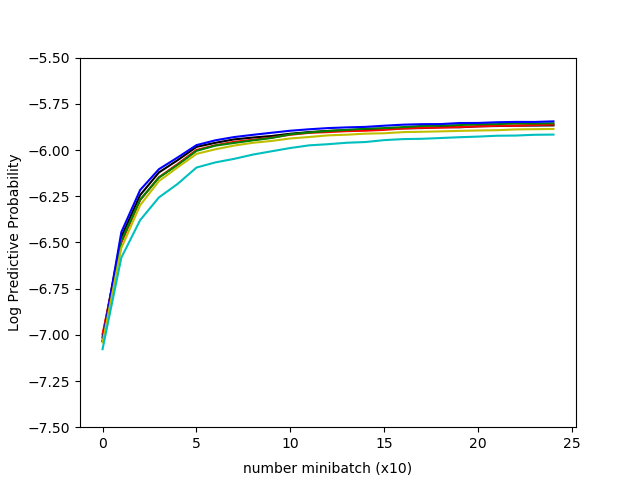
\includegraphics[width=1.1\textwidth]{Twitter_100gibb.png}}
		\end{figure}
	\end{column} %
	\hfill%	
	\begin{column}{.50\textwidth}
		\begin{figure}
			\subfloat[Online VB]{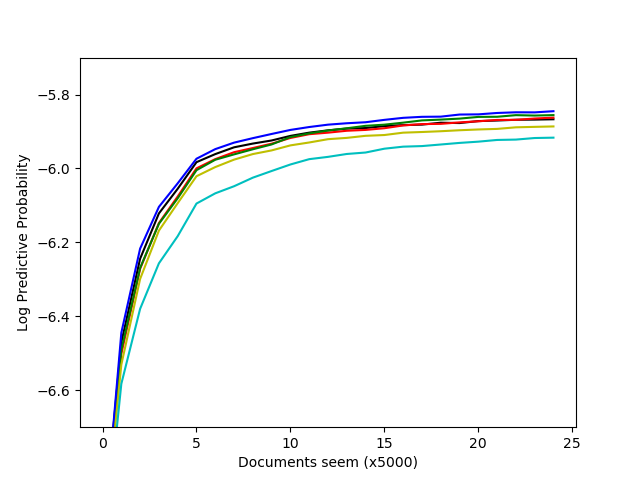
\includegraphics[width=1.1\textwidth]{Twitter_100vb.png}}
		\end{figure}				
	\end{column} %
\end{columns}
\begin{center}
	
\includegraphics[width=1\textwidth]{menu.png}	
\end{center}
\end{frame}

\begin{frame}{Tập dữ liệu Tweets, K = 100, sử dụng độ đo NPMI }
\begin{columns}[T] % align columns
\begin{column}{.50\textwidth}
	\begin{figure}
		\subfloat[Online Gibbs sampling]{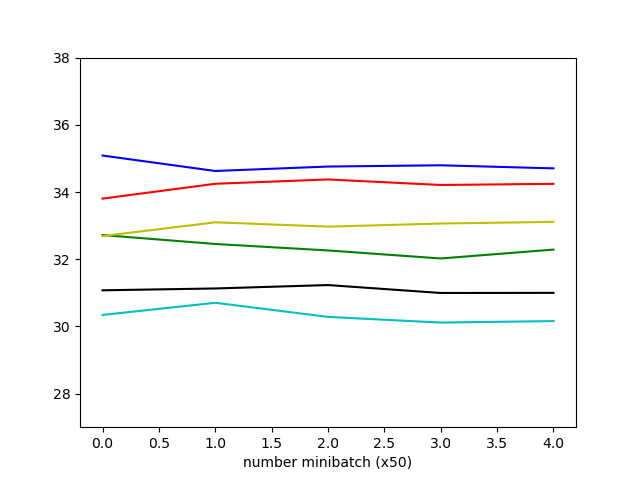
\includegraphics[width=1.1\textwidth]{Twitter_NPMI100gibb.png}}
	\end{figure}
\end{column} %
\hfill%	
\begin{column}{.50\textwidth}
	\begin{figure}
		\subfloat[Online VB]{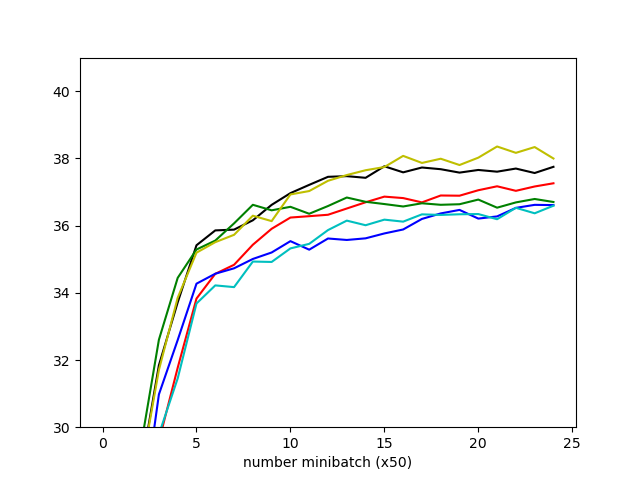
\includegraphics[width=1.1\textwidth]{Twitter_NPMI100vb.png}}
	\end{figure}				
\end{column} %
\end{columns}
\begin{center}

\includegraphics[width=1\textwidth]{menu.png}	
\end{center}
\end{frame}


\begin{frame}{Thời gian chạy với bộ dữ liệu Tweets}
		\begin{tabular}{l|c |c | c | c | c | c | c }
		drop rate & K & 0  & 0.1 & 0.3 & 0.5 & 0.7 & 0.9 \\
		 \arrayrulecolor{blue}\hline \hline
		\arrayrulecolor{black}
		Gibbs &50 & 249935& 231575 & 186822 & 80132 & 56739 & 24534 \\ 
%		\hline
		VB &50 & 3592& 3463 & 2922 & 2166 &1249 & 375 \\
		 \arrayrulecolor{blue}\hline \hline
		\arrayrulecolor{black}
		Gibbs &100 &404573 & 357891 & 288019 & 213525 & 134510&  46840\\ 
%		\hline
		VB &100 &3224 & 3050 & 2503 & 1870 &1189 &880\\
		 \arrayrulecolor{blue}\hline \hline
		\arrayrulecolor{black}
		Gibbs &150 &460189 & 429685 & 350120 & 297817 & 296984& 114108 \\ 
%		\hline
		VB &150 &3866 & 3696 & 3052 & 2429 &1536 &781\\
		 \arrayrulecolor{blue}\hline \hline
		\arrayrulecolor{black}
		Gibbs &200 & 539904& 538529 & 456806 & 387955 & 275327 & 171603 \\ 
%		\hline
		VB &200 &4925 & 4594 & 3313 & 2622 & 1944&1322
	\end{tabular}
\end{frame}

\begin{frame}{Tập dữ liệu Yahoo, K =100, độ đo perplexity}
%	K = 100, sử dụng độ đo perplexity 
	\begin{columns}[T] % align columns
		\begin{column}{.50\textwidth}
		\begin{figure}
			\subfloat[Online Gibbs sampling]{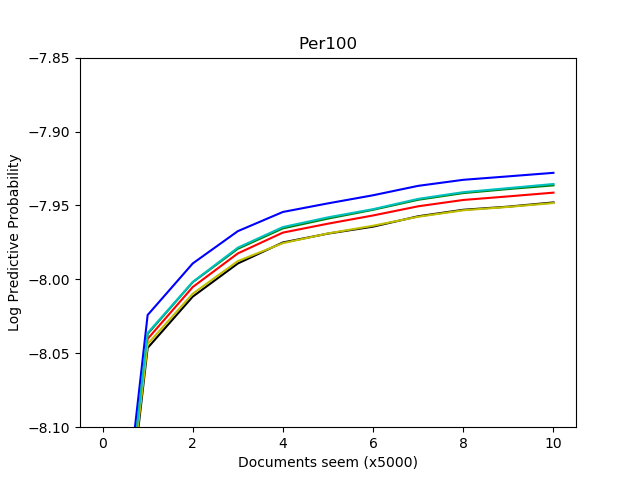
\includegraphics[width=1.1\textwidth]{yahoo100gibb.png}}
		\end{figure}
		\end{column} %
		\hfill%	
		\begin{column}{.50\textwidth}
			\begin{figure}
				\subfloat[Online VB]{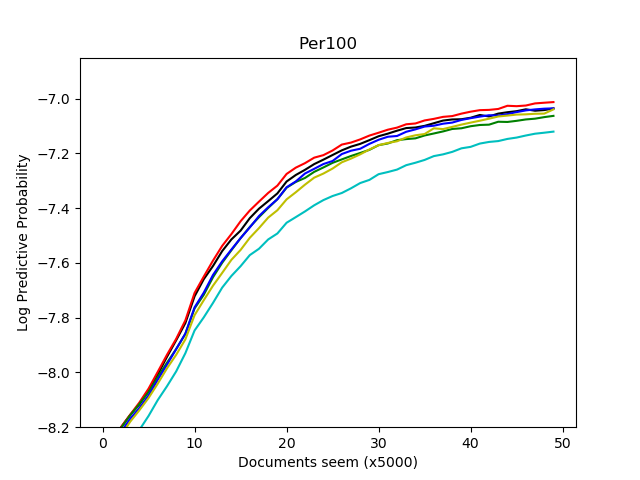
\includegraphics[width=1.1\textwidth]{yahoo100vb.png}}
			\end{figure}				
		\end{column} %
	\end{columns}
\begin{center}
	
\includegraphics[width=1\textwidth]{menu.png}	
\end{center}
\end{frame}

\begin{frame}{Tập dữ liệu Yahoo, K = 100, sử dụng độ đo NPMI }
\begin{columns}[T] % align columns
	\begin{column}{.50\textwidth}
		\begin{figure}
			\subfloat[Online Gibbs sampling]{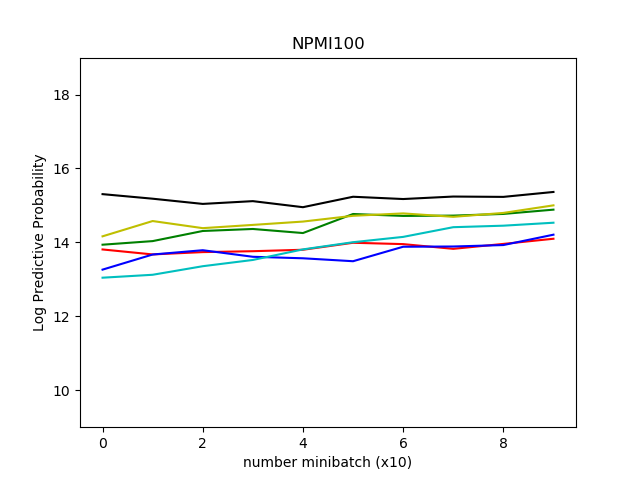
\includegraphics[width=1.1\textwidth]{yahoo_npmi100gibb.png}}
		\end{figure}
	\end{column} %
	\hfill%	
	\begin{column}{.50\textwidth}
		\begin{figure}
			\subfloat[Online VB]{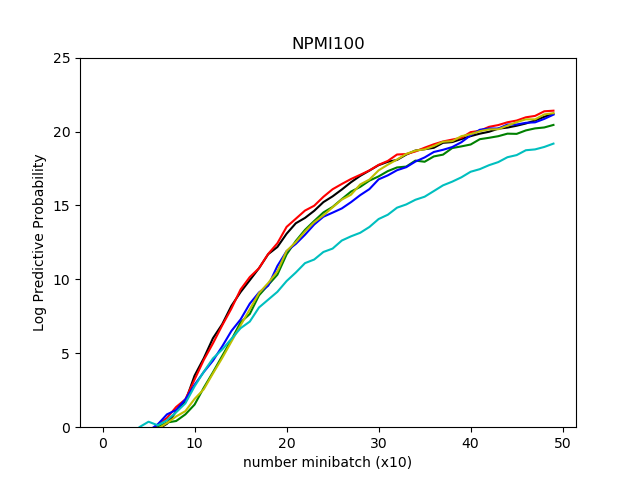
\includegraphics[width=1.1\textwidth]{yahoo_npmi100vb.png}}
		\end{figure}				
	\end{column} %
\end{columns}
\begin{center}
	
\includegraphics[width=1\textwidth]{menu.png}	
\end{center}
\end{frame}

\begin{frame}{Thời gian chạy với bộ dữ liệu Yahoo}
\begin{tabular}{l|c |c | c | c | c | c | c }
	drop rate & K & 0  & 0.1 & 0.3 & 0.5 & 0.7 & 0.9 \\
	\arrayrulecolor{blue}\hline \hline
	\arrayrulecolor{black}
	Gibbs &50 & 24259& 22605 & 18919 & 14154 & 9594 & 3856 \\ 
	%		\hline
	VB &50 & 3592& 3463 & 2922 & 2166 &1249 & 375 \\
	\arrayrulecolor{blue}\hline \hline
	\arrayrulecolor{black}
	Gibbs &100 &32042 & 27544 & 21763 & 16729 & 19533&  7565\\ 
	%		\hline
	VB &100 &448 & 418 & 372 & 328 &274 &223\\
	\arrayrulecolor{blue}\hline \hline
	\arrayrulecolor{black}
	Gibbs &150 &73385 & 68762 & 58344 & 44619 & 30748& 12387 \\ 
	%		\hline
	VB &150 &514 & 490 & 453 & 398 &337 &265\\
	\arrayrulecolor{blue}\hline \hline
	\arrayrulecolor{black}
	Gibbs &200 & 64068& 51862 & 46133 & 6406 & 41653 & 8894 \\ 
	%		\hline
	VB &200 &580 & 559 & 485 & 434 & 373 &306
\end{tabular}
\end{frame}

\begin{frame}{Tập dữ liệu NYT, K = 100, sử dụng độ đo perplexity }

\begin{columns}[T] % align columns
	\begin{column}{.50\textwidth}
		\begin{figure}
			\subfloat[Online Gibbs sampling]{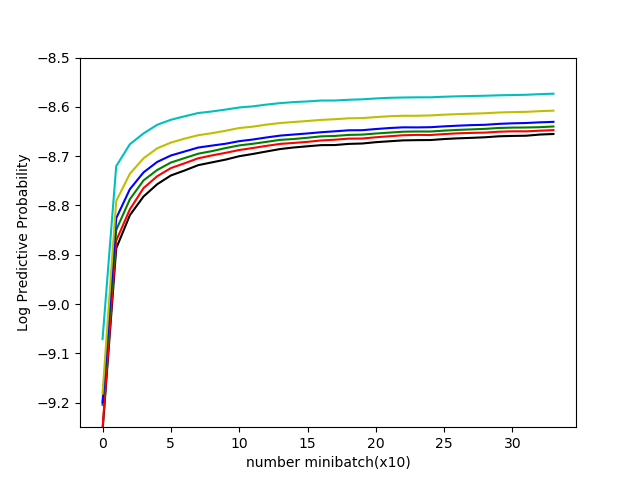
\includegraphics[width=1.1\textwidth]{nyt100gibb.png}}
		\end{figure}
	\end{column} %
	\hfill%	
	\begin{column}{.50\textwidth}
		\begin{figure}
			\subfloat[Online VB]{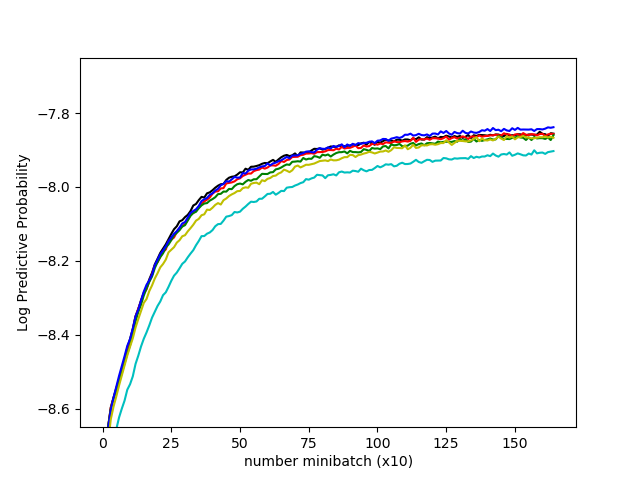
\includegraphics[width=1.1\textwidth]{nyt100vb.png}}
		\end{figure}				
	\end{column} %
\end{columns}
\begin{center}
	
\includegraphics[width=1\textwidth]{menu.png}	
\end{center}
\end{frame}


\begin{frame}{Tập dữ liệu NYT, K = 100, sử dụng độ đo NPMI }
\begin{columns}[T] % align columns
	\begin{column}{.50\textwidth}
		\begin{figure}
			\subfloat[Online Gibbs sampling]{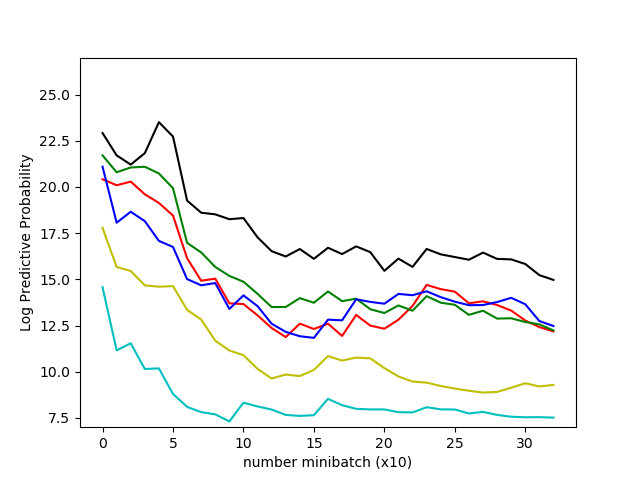
\includegraphics[width=1.1\textwidth]{npmi_nyt_100_gibbs.png}}
		\end{figure}
	\end{column} %
	\hfill%	
	\begin{column}{.50\textwidth}
		\begin{figure}
			\subfloat[Online VB]{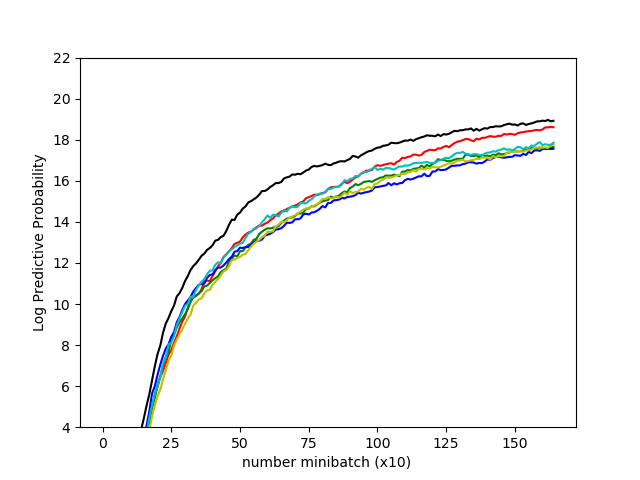
\includegraphics[width=1.1\textwidth]{npmi_nyt_100_vb.png}}
		\end{figure}				
	\end{column} %
\end{columns}
\begin{center}
	
\includegraphics[width=1\textwidth]{menu.png}	
\end{center}
\end{frame}


\begin{frame}{Thời gian chạy với bộ dữ liệu NYT}
\begin{tabular}{l|c |c | c | c | c | c | c }
	drop rate & K & 0  & 0.1 & 0.3 & 0.5 & 0.7 & 0.9 \\
	\arrayrulecolor{blue}\hline \hline
	\arrayrulecolor{black}
	Gibbs &50 & 81029& 75909 & 63424 & 49757 & 33146 & 11787 \\ 
	%		\hline
	VB &50 & 3592& 3463 & 2922 & 2166 &1249 & 375 \\
	\arrayrulecolor{blue}\hline \hline
	\arrayrulecolor{black}
	Gibbs &100 &90219 & 85610 & 71573 & 56306 & 39515&  15900\\ 
	%		\hline
	VB &100 &3224 & 3050 & 2503 & 1870 &1189 &880\\
	\arrayrulecolor{blue}\hline \hline
	\arrayrulecolor{black}
	Gibbs &150 &130083 & 123790 & 124131 & 107083& 89761& 38267 \\ 
	%		\hline
	VB &150 &3866 & 3696 & 3052 & 2429 &1536 &781\\
	\arrayrulecolor{blue}\hline \hline
	\arrayrulecolor{black}
	Gibbs &200 & 193110& 180111 & 184658 & 151754 & 47640 & 33396 \\ 
	%		\hline
	VB &200 &4925 & 4594 & 3313 & 2622 & 1944&1322
\end{tabular}
\end{frame}

\begin{frame}{Đánh giá}
	\begin{itemize}
		\item Phương pháp Gibbs sampling
		\begin{itemize}
			\item Thời gian chạy rất chậm.
			\item Sử dụng phương pháp học ngẫu nhiên cho kết quả xấp xỉ nhau nhưng thời gian cải thiện rất đáng kể.
		\end{itemize}
		\item Phương pháp VB cho thời học rất nhanh, và kết quả cao hơn so với phương pháp học Gibbs sampling
	\end{itemize}
\end{frame}
%%%%%%%%%%%%%%%%%%%%%%%%%%%%%%%%%%%%%%%%%%%
\section{Kết luận}
	\begin{frame}{Kết luận}
		\begin{itemize}
			\item Hai phương pháp học mới:
			\begin{itemize}
				\item Phương pháp học VB \\=> Cho kết quả cao hơn và thời gian nhanh hơn rất nhiều so với  phương pháp Gibbs sampling
				\item Phương pháp học ngẫu nhiên \\=> Cải thiện thời gian học rất đáng kể
			\end{itemize}
		\end{itemize}
	\end{frame}

%%%%%%%%%%%%%%%%%%%%%%%%%%%%%%%%%%%%%%%%%%%
%\section{Phụ lục}
%
%\begin{frame}{Tập dữ liệu Tweets, K =50, đô đo perplexity}
%%	K = 100, sử dụng độ đo perplexity 
%\begin{columns}[T] % align columns
%	\begin{column}{.50\textwidth}
%		\begin{figure}
%			\subfloat[Online Gibbs sampling]{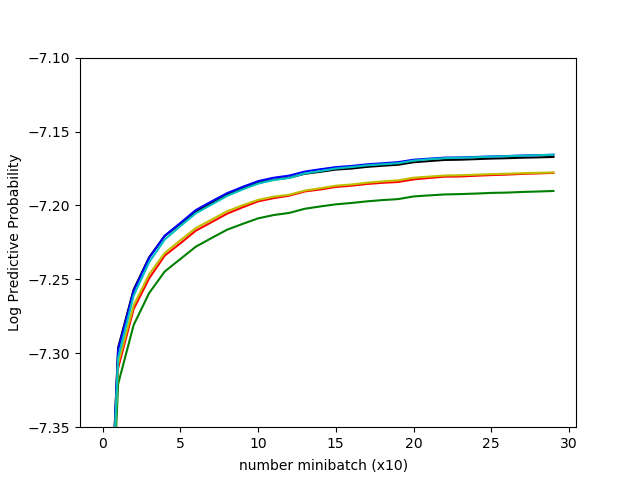
\includegraphics[width=1.1\textwidth]{Twitter_50gibb.png}}
%		\end{figure}
%	\end{column} %
%	\hfill%	
%	\begin{column}{.50\textwidth}
%		\begin{figure}
%			\subfloat[Online VB]{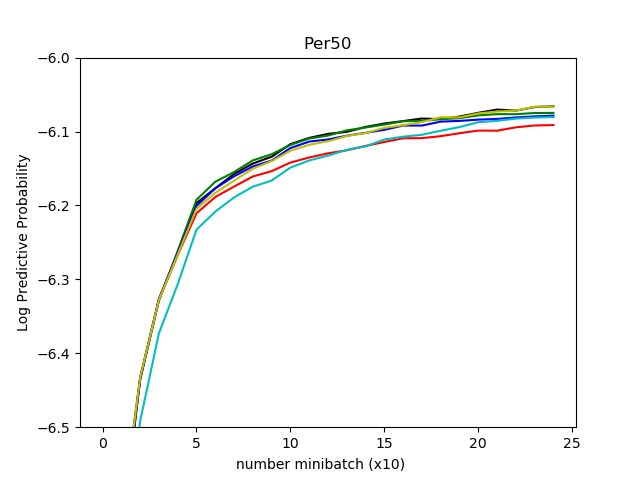
\includegraphics[width=1.1\textwidth]{Twitter_50vb.png}}
%		\end{figure}				
%	\end{column} %
%\end{columns}
%\begin{center}
%	
\includegraphics[width=1\textwidth]{menu.png}	
%\end{center}
%\end{frame}
%
%\begin{frame}{Tập dữ liệu Tweets, K = 50, sử dụng độ đo NPMI }
%\begin{columns}[T] % align columns
%\begin{column}{.50\textwidth}
%	\begin{figure}
%		\subfloat[Online Gibbs sampling]{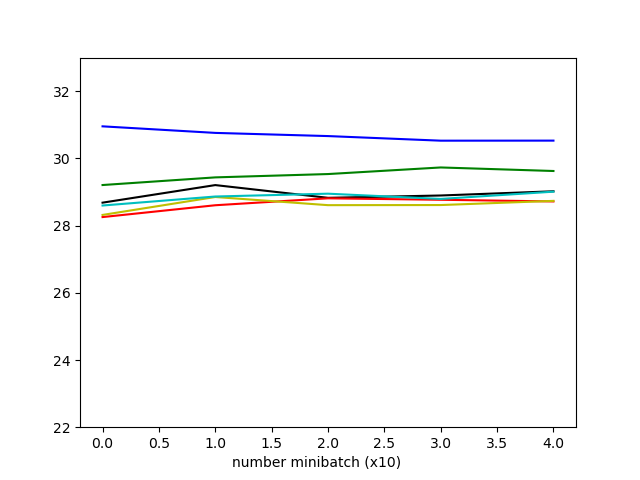
\includegraphics[width=1.1\textwidth]{Twitter_NPMI50gibb.png}}
%	\end{figure}
%\end{column} %
%\hfill%	
%\begin{column}{.50\textwidth}
%	\begin{figure}
%		\subfloat[Online VB]{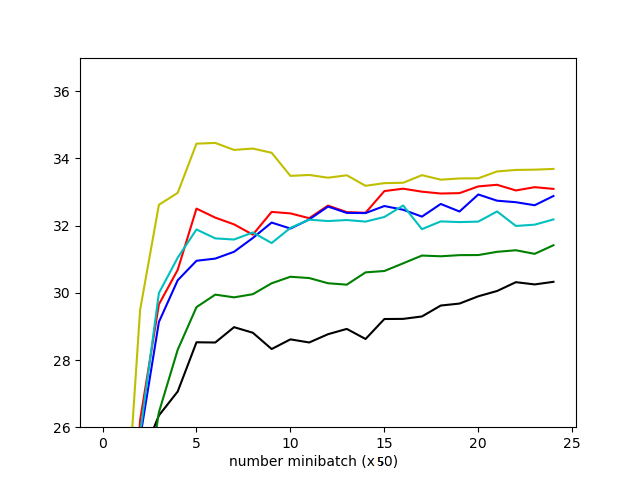
\includegraphics[width=1.1\textwidth]{Twitter_NPMI50vb.png}}
%	\end{figure}				
%\end{column} %
%\end{columns}
%\begin{center}
%
\includegraphics[width=1\textwidth]{menu.png}	
%\end{center}
%\end{frame}
%
%
%\begin{frame}{Tập dữ liệu Tweets, K =150, đô đo perplexity}
%%	K = 100, sử dụng độ đo perplexity 
%\begin{columns}[T] % align columns
%	\begin{column}{.50\textwidth}
%		\begin{figure}
%			\subfloat[Online Gibbs sampling]{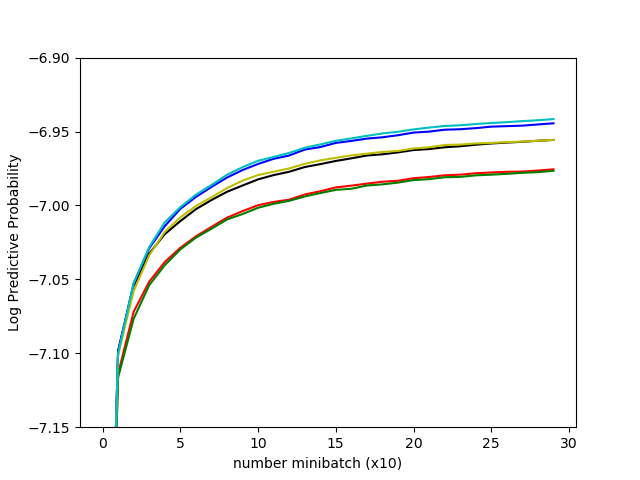
\includegraphics[width=1.1\textwidth]{Twitter_150gibb.png}}
%		\end{figure}
%	\end{column} %
%	\hfill%	
%	\begin{column}{.50\textwidth}
%		\begin{figure}
%			\subfloat[Online VB]{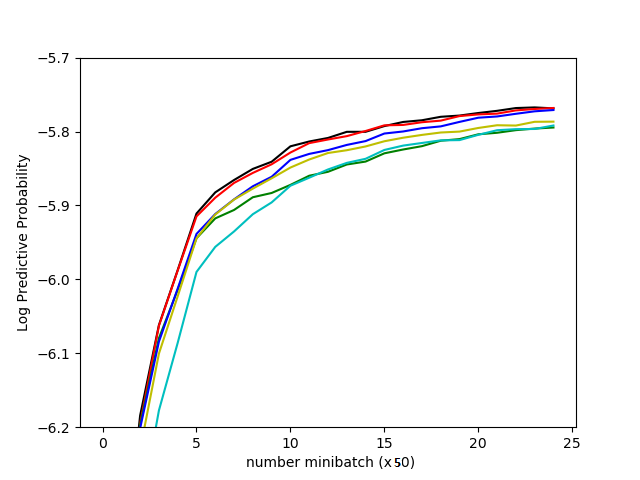
\includegraphics[width=1.1\textwidth]{Twitter_150vb.png}}
%		\end{figure}				
%	\end{column} %
%\end{columns}
%\begin{center}
%	
\includegraphics[width=1\textwidth]{menu.png}	
%\end{center}
%\end{frame}
%
%
%\begin{frame}{Tập dữ liệu Tweets, K =200, đô đo perplexity}
%%	K = 100, sử dụng độ đo perplexity 
%\begin{columns}[T] % align columns
%	\begin{column}{.50\textwidth}
%		\begin{figure}
%			\subfloat[Online Gibbs sampling]{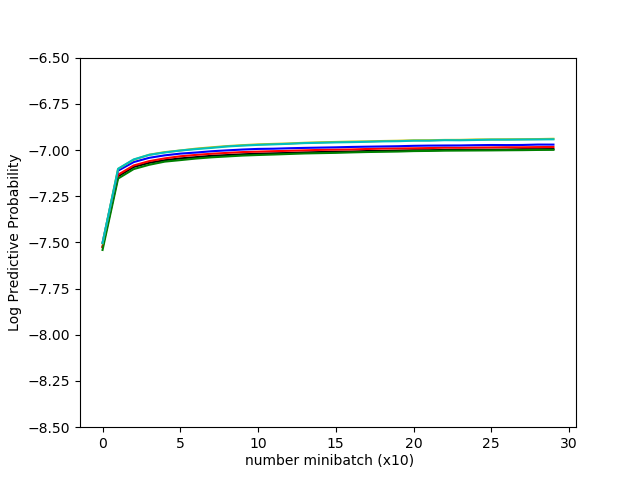
\includegraphics[width=1.1\textwidth]{Twitter_200gibb.png}}
%		\end{figure}
%	\end{column} %
%	\hfill%	
%	\begin{column}{.50\textwidth}
%		\begin{figure}
%			\subfloat[Online VB]{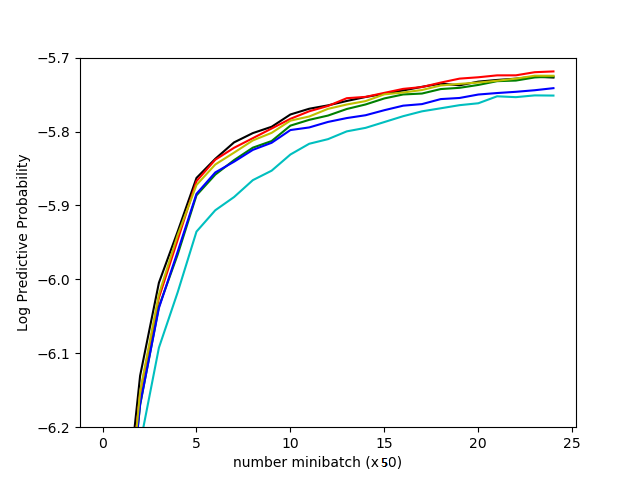
\includegraphics[width=1.1\textwidth]{Twitter_200vb.png}}
%		\end{figure}				
%	\end{column} %
%\end{columns}
%\begin{center}
%	
\includegraphics[width=1\textwidth]{menu.png}	
%\end{center}
%\end{frame}
%
%\begin{frame}{Tập dữ liệu Tweets, K = 50, sử dụng độ đo NPMI }
%\begin{columns}[T] % align columns
%	\begin{column}{.50\textwidth}
%		\begin{figure}
%			\subfloat[Online Gibbs sampling]{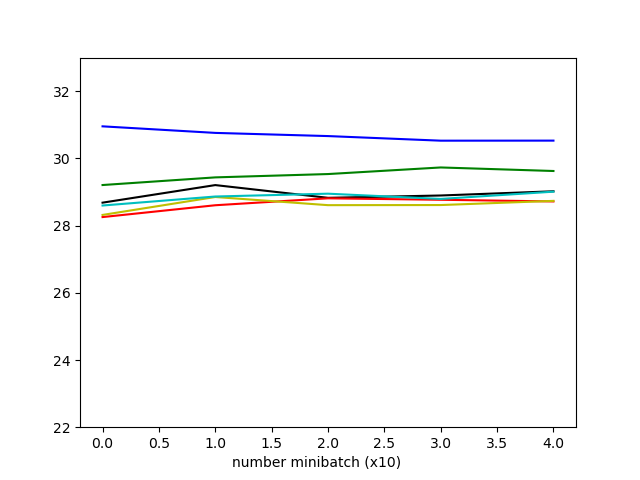
\includegraphics[width=1.1\textwidth]{Twitter_NPMI50gibb.png}}
%		\end{figure}
%	\end{column} %
%	\hfill%	
%	\begin{column}{.50\textwidth}
%		\begin{figure}
%			\subfloat[Online VB]{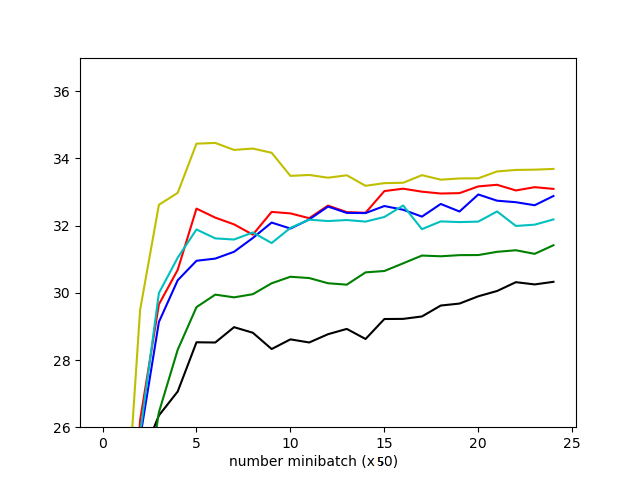
\includegraphics[width=1.1\textwidth]{Twitter_NPMI50vb.png}}
%		\end{figure}				
%	\end{column} %
%\end{columns}
%\begin{center}
%	
\includegraphics[width=1\textwidth]{menu.png}	
%\end{center}
%\end{frame}


\end{document}
